\subsection{Working Description}

 image preprocessing paragraph.\\

Before feeding an image into the model, it undergoes essential preprocessing to ensure compatibility. This includes converting the image into numeric vectors, a step known as input embedding. This process is crucial for aligning raw image data with the Vision Transformer (ViT) architecture. The image is divided into non-overlapping patches, each undergoing linear embedding to create fixed-size vectors. This transforms the image into a sequential arrangement of vectors, enabling sequential processing by the transformer model.\\

Initially, the input image undergoes segmentation into patches, a necessary step to conform with the sequential processing design of transformers. The formulation of these patches considers factors such as the image's height, width, color channels (red, green, and blue), and the batch size for multiple images. The input image, characterized by specific dimensions in terms of height and width, three color channels, and an optional batch dimension for multiple images, is thus transformed into a sequence to align with the architecture of transformers.\\
\begin{figure}[htbp]
    \centering
    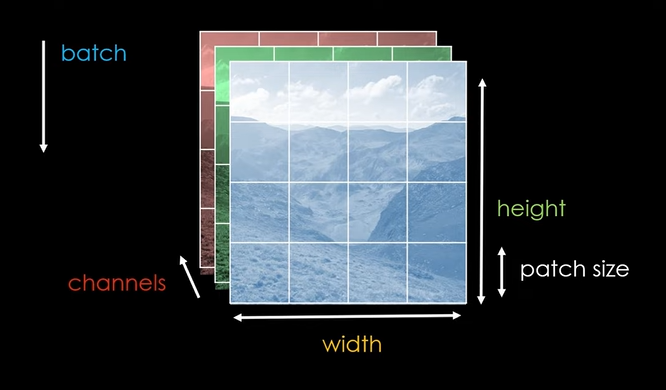
\includegraphics[width=4in]{img/colorbatch.png}
    \caption{\textit{Image with RGB color channels}}
\end{figure}\\
The images undergo resizing and conversion into tensors, representing the initial phase of the process. Following this, the "PatchEmbedding" module is employed to reshape the tensors. This reshaping step plays a pivotal role, setting the stage for a linear transformation that ultimately yields embedding vectors. A linear transformation was utilized on flattened image patches of one-dimensional sequence, to map them to a desired dimension.\\

Einops-Einstein Operation, is a Python library that was used which simplifies tensor operations. Inspired by Einstein summation conventions, it offers an expressive syntax for reshaping and reducing and manipulation of tensors. \\

After completing the patching process, the original positions of the patches within an image becomes unknown. To address this, position embedding is employed. Since the attention mechanism in transformers is position-independent, position embedding is introduced to enable the model to comprehend the specific locations of each patch in the original image. A vector is assigned to each patch, representing its unique position within the image. The values within these position embedding vectors are derived from sine and cosine functions.\\
The formula for positional encoding is as follows:\\
\\
\[
PE_{(pos, 2i)} = \sin\left(\frac{pos}{{10000}^{(2i/d)}}\right)
\]

\[
PE_{(pos, 2i+1)} = \cos\left(\frac{pos}{{10000}^{(2i/d)}}\right)
\]
\\
Where:
\begin{align*}
    \text{pos} & : \text{the position of the token in the sequence.} \\
    i & : \text{the dimension of the positional encoding.} \\
    d & : \text{the dimension of the model or embedding.}
\end{align*}

\begin{figure}[htbp]
    \centering
    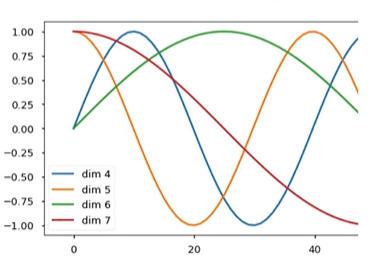
\includegraphics[width=4in]{img/plot for sine and cosine wave.png}
    \caption{\textit{Value vs Position graph for sine and cosine wave}}
\end{figure}

\begin{figure}[htbp]
    \centering
    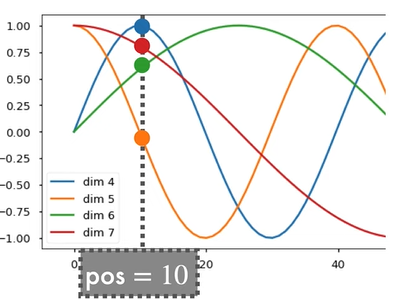
\includegraphics[width=4in]{img/pos 10.png}
    \caption{\textit{Graph for sine and cosine wave  at position 10}}
\end{figure}
For a patch at position 10, the values in its associated position embedding vectors is equivalent to to corresponding values intersecting within the curve as shown in the graph.\\

In the process of adding position embeddings to an image, we introduced a special vector known as the CLS token, where CLS stands for Classification Token. The CLS token is a unique vector assigned to each input image. Initially, it receives random values and is considered a placeholder. However, as the model learns, these values are adjusted based on the information gathered from all other input patches. This adjustment process makes the CLS token a "learnable vector," as it evolves during training to contribute valuable information for the classification task.

\begin{figure}[htbp]
    \centering
    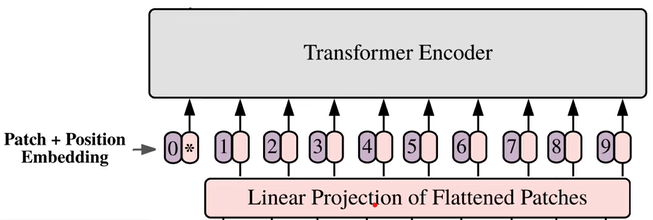
\includegraphics[width=5in]{img/CLS token.png}
    \caption{\textit{CLS Token and position embedding vectors}}
\end{figure}

The CLS token functions as a universal feature extractor, capturing the essence of the entire image. This extracted information can then be utilized for various tasks downstream. The learning positional embeddings helps reduce inductive biases. These embeddings are added on top of input embedding vectors and are not concatenated with them.\\
\\
The Embedded Patches are then passed onto the Encoder section of the model.\\
\begin{figure}[htbp]
    \centering
    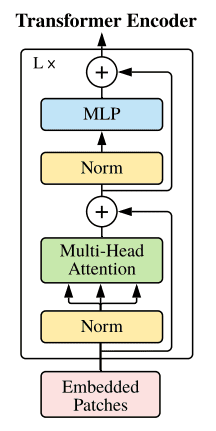
\includegraphics[width=2in]{img/encoderblock.png}
    \caption{\textit{Transformer Encoder}}
\end{figure}\\

Multihead attention is a mechanism designed to capture different aspects or relationships within input sequences. It involves splitting the input into multiple heads or sets, each with its own set of learned weights. The attention mechanism is then applied independently to each head in parallel.
The multihead attention is the scaled dot product attention mechanism of the transformer and allows to share info between different inputs.\\

In multihead attention, there are three primary inputs:\\

\textbf{Query (Q):} This represents the set of queries used to retrieve information from the input sequence. It is usually derived from the input data and is transformed to capture relevant features.\\

\textbf{Key (K):} The key input consists of keys associated with each element in the input sequence. Like the query, it is derived from the input data and aims to provide information about the relationships between different elements.\\

\textbf{Value (V):} The value input includes the values or content associated with each element in the input sequence. It also comes from the input data and provides the actual information that will be weighted and combined based on the attention mechanism.\\

The Multihead attention process is also regarded as the process where there is inter linkage between the inputs such that exchange of information takes place. To put these Q, K and V to a simple understanding, value is the component that actually is communicated in multihead attention process, query is equivalent for "what i am looking for" and key is equivalent for "what i have."\\

For further explanation  on Multihead Attention, suppose we have inputs to attention blocks of N embeddings (total N+1 including CLS token) and dimension D. With the help of N and D, a stacked matrix can be obtained.
\[ X \in \mathbb{R}^{N \times D}\] 

For a single head attention we project each patch embeddings for 3 separate iteration to produce the key, queries and values. The three matrices to produce the keys, queries and values would be:
\[ W^Q \in \mathbb{R}^{D\times d_k}\] 
\[ W^K \in \mathbb{R}^{D \times d_k}\] 
\[ W^V \in \mathbb{R}^{D \times d_v}\] 
Where:
\begin{align*}
    d_k & : \text{the dimension of query and key .} \\
    d_v & : \text{the dimension of values.}
\end{align*}
Therefore, the key(K), query(Q) and value(V) can be obtained when the original embedding matrix X is multiplied with the above mentioned matrices.
\[Q = X.W^Q \in \mathbb{R}^{N\times d_k}\] 
\[K = X.W^K \in \mathbb{R}^{N\times d_k}\] 
\[V = X.W^V \in \mathbb{R}^{N\times d_v}\] \\

The multihead attention will contain 'h' numbers of heads, each head representing as a single. All these multiple heads undergo computation in parallel. \\

The general form of  scaled dot-product attention is given as:
\[\text{Attention}(h) = \text{softmax}\left(\frac{Q_h * K_h ^T}{\sqrt{d_k}}\right) V_h\]
The softmax is applied along the rows of the matrix to normalize them to probability vectors and $d_k$ helps in avoiding peaky affinities.When attention distributions are too peaky, it suggests the model is assigning a significantly higher weight to a small subset of elements in the input sequence while largely ignoring the rest.\\

Finally, \[\text{Multihead Attention} = \text{concat} (h_1, h_2, h_3,...,H)* W^o \]

$W^0$ is added to ensure the right dimension is obtained.\\

The asymptotic complexity, often denoted as Big O notation, for Multi-Head Attention (MHA) in the Transformer model is typically expressed as\[ O(N \cdot d^2 \cdot H)\], where:
\begin{itemize}
  \item $N$ is the sequence length,
  \item $d$ is the dimensionality of the model's hidden representations,
  \item $H$ is the number of attention heads.
\end{itemize}
Because of this when processing long sequences, the computational cost of Multihead Attention, can be substantial.\\

At present context, multihead attention doesn't require building from scratch; instead, it can be accessed through a pre-existing module.

\paragraph*{This section in Raw}
Pytorch implementation of multihead attention block.
self.q=torch.nn.linear(dim,dim)\\
q,k,v are obtained after linear transformation
then image is passed through a function as 
def forward=(self,img)\\
q=self.q(img)


and then attention output is obtained as self.att(q,k,v)

Layer Normalization: normalizes all input in a layer for each individual sample

PreNorm is used for Normalization

Takes the attention function and apply Normalization.\\
\\

Feed Forward  Networks (FFN):
linear\\
GELU\\
Dropout\\
linear\\
Dropout -> used to avoid over fitting\\
\\
Residual (skip connection)
Used to improve flow of info 
Omit vanishing gradient (loss of training signals during back propagation)





\newpage